\documentclass[11pt]{article}

\usepackage[margin=0.95in]{geometry}
\usepackage[utf8]{inputenc}
\usepackage[T1]{fontenc}
\usepackage{lmodern}
\usepackage{microtype}
\usepackage{xcolor}
\usepackage{titlesec}
\usepackage{enumitem}
\usepackage{tcolorbox}
\tcbuselibrary{skins,breakable}
\usepackage{tikz}
\usetikzlibrary{arrows.meta, positioning, calc, shapes.geometric}
\usepackage{hyperref}
\usepackage{fancyhdr}
\usepackage{ragged2e}
\usepackage{parskip}

\definecolor{accent}{HTML}{1D4E6B}
\definecolor{accentdeep}{HTML}{102E40}
\definecolor{accentlight}{HTML}{EAF2F7}
\definecolor{warn}{HTML}{8A5A1C}
\definecolor{warnlight}{HTML}{FBF1E3}
\definecolor{good}{HTML}{2C6B4F}
\definecolor{goodlight}{HTML}{EAF5EF}
\definecolor{textgray}{HTML}{2B2B2B}

\hypersetup{
    colorlinks=true,
    linkcolor=accent,
    citecolor=accent,
    urlcolor=accent
}

\color{textgray}

\titleformat{\section}
  {\color{accentdeep}\Large\bfseries}
  {\thesection}{0.6em}{}
\titlespacing{\section}{0pt}{1.4em}{0.6em}
\titleformat{\subsection}
  {\color{accent}\large\bfseries}
  {\thesubsection}{0.5em}{}
\titlespacing{\subsection}{0pt}{1em}{0.4em}

\pagestyle{fancy}
\fancyhf{}
\renewcommand{\headrulewidth}{0pt}
\fancyfoot[C]{\small\color{gray} Understanding Is Not Observable \quad$\cdot$\quad \thepage}

\newtcolorbox{statbox}[1][]{
  colback=accentlight, colframe=accent, boxrule=0.6pt, arc=2pt,
  left=8pt, right=8pt, top=6pt, bottom=6pt, #1
}
\newtcolorbox{pullquote}[1][]{
  enhanced, colback=white, colframe=white, boxrule=0pt,
  left=18pt, right=18pt, top=4pt, bottom=4pt,
  borderline west={3pt}{0pt}{accent}, #1
}
\newtcolorbox{provenbox}[1][]{
  colback=goodlight, colframe=good, boxrule=0.6pt, arc=2pt,
  left=8pt, right=8pt, top=6pt, bottom=6pt, #1
}
\newtcolorbox{opennbox}[1][]{
  colback=warnlight, colframe=warn, boxrule=0.6pt, arc=2pt,
  left=8pt, right=8pt, top=6pt, bottom=6pt, #1
}

\begin{document}

% ---------- TITLE PAGE ----------
\begin{titlepage}
\centering
\vspace*{1.6cm}

{\color{accent}\rule{0.5\textwidth}{1.2pt}}

\vspace{1.4cm}
{\Huge\bfseries\color{accentdeep} Understanding Is\\[2pt] Not Observable}

\vspace{0.8cm}
{\Large\color{accent} Why you can't tell if two minds actually connect --- and what to do instead}

\vspace{1.6cm}
{\color{accent}\rule{0.5\textwidth}{1.2pt}}

\vspace{2.2cm}
{\large A working paper, a proof, and an open next step}

\vspace{0.5cm}
{\normalsize\color{gray} Ashok Pasala \quad $\cdot$ \quad Snigdha Gorai \\ VIT-AP University \\ August 2026}

\vfill

\begin{tcolorbox}[colback=accentlight, colframe=accent, width=0.82\textwidth, arc=3pt, boxrule=0.6pt]
\centering\normalsize
\textbf{In one sentence:} you cannot tell whether two systems understand each other by watching them --- only by testing it --- and almost nobody currently tests it that way.
\end{tcolorbox}

\vspace{1.2cm}
\end{titlepage}

% ---------- BODY ----------

\section*{A horse that could do arithmetic}
\addcontentsline{toc}{section}{A horse that could do arithmetic}

A horse named Clever Hans could supposedly solve arithmetic. Ask him ``what's four plus three?'' and he'd tap his hoof seven times and stop. Crowds came. Scientists tested him and, for years, could not catch him cheating.

Then someone asked the question without letting the questioner know the answer either. Hans's accuracy collapsed instantly. He had never been doing math --- he was reading the tiny, involuntary tension in a human body relaxing the moment the correct tap count was reached. Everyone watching, including the scientists, had mistaken a very convincing imitation of understanding for the real thing, because the only tool anyone had was watching.

\begin{pullquote}
\textit{This project found a modern, provable, much larger version of the same problem --- and a test that actually catches it.}
\end{pullquote}

\section{Where it started}

Human speech carries roughly \textbf{39 bits of information per second}, remarkably consistent across seventeen languages spanning nine language families. Deliberate human behaviour more broadly has been measured at around \textbf{10 bits per second}. The sensory periphery, meanwhile, takes in information roughly a \textbf{billion} times faster. That gap is real, well measured, and has been sitting there the entire time anyone has studied communication.

The obvious idea: the mouth and the ear are the bottleneck. Build a direct brain-to-brain link, skip articulation and hearing entirely, and two minds should finally exchange information at something closer to their true internal speed.

We did not merely hold that idea --- we built the piece the field was missing. Brain-connection hardware has been designed for a decade without anyone defining what quantity such a link is supposed to \emph{maximise}, rather as if modems had been engineered before Shannon defined channel capacity in 1948. So we defined one: \textbf{coupling capacity}, a measure of how far one system's signal can steer another's internal trajectory. And we proved a theorem about it with a genuinely surprising ceiling --- set not by the width of the wire, but by the number of independent directions the \emph{receiver} can be moved along at all. Past a certain point, a wider channel buys nothing whatsoever.

That theorem is still true, and it is Section 2 of the paper. What happened next is why it is not the headline.

\section{The experiment that changed the premise}

We tested it properly, in a controlled system built for exactly this question: two learning agents, one that holds private information, one that needs to act on it, connected by a channel we fully control.

Then we ran the strongest possible version of ``remove the bottleneck.'' Not a wider channel --- \emph{no channel at all}. The first agent's private information was handed directly to the second: free, instant, perfect, zero noise, zero delay. The literal physical ceiling that no interface of any kind could ever exceed.

\begin{statbox}
\centering
\textbf{Result of the zero-bottleneck test}\\[4pt]
{\Large $-16.0$} \quad performance with the information handed over for free \\
{\Large $-16.9$} \quad performance with \emph{no} information at all\\
{\Large $-8.8$} \quad performance an agent that actually uses the information can reach
\end{statbox}

Handing over the information changed nothing. The receiver behaved exactly as if it had been told nothing at all, even with the most generous channel physically possible. The bottleneck was never the channel.

\section{What was actually missing}

Two systems can only communicate if they already agree, in advance, on what a given signal means. Not the wire --- the \emph{code}. A word only works because both sides already agreed, long before this sentence, roughly what it points to. The channel is the delivery truck; the shared agreement is the cargo that makes delivery worth anything.

That single fact has an uncomfortable consequence. If shared agreement is what makes communication work, shared agreement is also exactly what makes it \emph{impossible to check from the outside} whether real communication is happening at any given moment. A system genuinely tracking its partner's specific signal, and a system merely running the same shared code on autopilot without being moved by anything in particular right now, produce \textbf{identical} outside signatures --- same measured synchrony, same decodable information, same everything anyone currently watches for.

\begin{center}
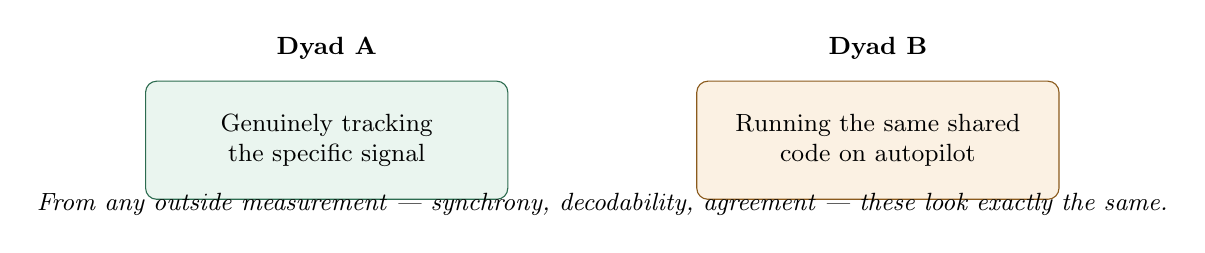
\begin{tikzpicture}[
  box/.style={draw, rounded corners, minimum width=4.6cm, minimum height=1.5cm, align=center, font=\small},
  lbl/.style={font=\small\bfseries}
]
\node[box, fill=goodlight, draw=good] (d1) at (0,0) {Genuinely tracking\\the specific signal};
\node[box, fill=warnlight, draw=warn] (d2) at (7,0) {Running the same shared\\code on autopilot};
\node[lbl, above=0.15cm of d1] {Dyad A};
\node[lbl, above=0.15cm of d2] {Dyad B};
\node[align=center, font=\small\itshape, below=0.55cm of $(d1)!0.5!(d2)$] {From any outside measurement --- synchrony, decodability, agreement --- these look exactly the same.};
\end{tikzpicture}
\end{center}

We proved this formally, and built a system where it can be seen directly with real numbers: a receiver whose internal state contained its partner's private goal almost perfectly (recoverable to an error of \textbf{0.0017}), while its actual behaviour used essentially none of it.

\section{So how much faster could this actually get?}

The question everyone asks. Here is the honest version, in one number and one caveat that has to travel with it.

\begin{statbox}
\centering
\textbf{The theoretical gap}\\[4pt]
{\Large $\sim 10^9$ bits/s} \quad senses \qquad vs \qquad {\Large $\sim 10$ bits/s} \quad deliberate behaviour\\[6pt]
{\large\bfseries up to a hundred-million-fold, unrealised}
\end{statbox}

\vspace{0.3cm}
That is the number that has quietly motivated a decade of brain-interface research, whether anyone said it out loud or not.

\begin{pullquote}
\textbf{The caveat, and it's the whole point of this project.} We ran the most direct test of that gap physically possible --- information handed over free, zero channel, zero noise, the best case any interface could ever achieve. It captured \textbf{zero percent} of it. Not a small percentage. Zero, statistically, measured. The mouth was never what was limiting it.
\end{pullquote}

\textbf{What's still open:} whether a \emph{different} kind of gain exists --- not from widening the channel, but from an interface that grows a shared convention between two systems over time. Nobody has measured how much of that gap such an interface could recover, because nobody has built and tested one yet. Real, open, and a different question entirely from ``how much faster is a wider pipe.''

\section{What survived the collapse, and what did not}

This is the part people ask about, and the part easiest to fudge, so it is worth stating precisely.

\textbf{The theorem survived.} A channel can drive a receiver along only as many independent directions as that receiver possesses. No quantity of bandwidth repairs that. It is proven, it is in the paper, and we would defend it.

\textbf{The measurement programme built on top of it did not.} Two reasons, both of which we found ourselves rather than had pointed out to us. First, the original validation ran in a simulation satisfying the theory's assumptions by construction --- in one case a coupling parameter was \emph{imposed} on the simulator and then recovered, and the match was reported as confirmation. That demonstrates the measuring instrument inverts the model. It is not evidence for the theory, and presenting it as such was an overstatement we have since corrected in print. Second, and more seriously: the quantity the programme was designed to measure is precisely the quantity we later proved cannot be measured by observation.

\begin{pullquote}
\textit{An unused channel is trivially consistent with any upper bound on what it could have carried. We had built a ceiling for something that was sitting at zero for reasons the ceiling had nothing to say about.}
\end{pullquote}

\section{Why this is bigger than one experiment}

This exact blind spot is quietly built into how several fields currently check for understanding.

\subsection*{AI evaluation}
Chatbots and AI assistants are tested by watching them talk --- benchmarks, preference scores, dialogue quality. If ``looks right'' and ``is actually tracking what you meant'' are indistinguishable from outside, a large share of current AI evaluation is measuring the wrong thing, the same way watching Hans tap was the wrong test.

\subsection*{Neuroscience}
``Brain synchrony'' between two interacting people is routinely reported as evidence of connection. The same blind spot applies: synchronized activity and functioning understanding are not the same measurement, and the field has not had a clean way to separate them.

\subsection*{Brain-computer interfaces}
Between 2014 and 2019, brain-interface hardware improved substantially --- and the amount of information actually transmitted \emph{fell}, from roughly 0.25--0.81 bits per trial down to 0.336. The field's own researchers noted this without an explanation. Once the bottleneck is understood to be shared convention rather than hardware, the anomaly stops being an anomaly.

\begin{opennbox}
\textbf{Independent support, found after the fact.} A 2024/2025 \textit{Neuron} paper (Zheng \& Meister, Caltech) independently confirmed the $\sim$10 bits/s behavioural ceiling. A 2026 peer-reviewed \textit{Journal of Neural Engineering} paper argues mainstream BCI's real constraint is an ``input/output disparity,'' not channel count. A 2024 hyperscanning paper found brain synchrony barely moves even when researchers directly control whether two people are seeing the same information. None of these use this framing --- but pieces of the same picture keep surfacing independently, which is what a real pattern looks like.
\end{opennbox}

\section{The fix}

You cannot find this gap by watching more carefully. You have to intervene: remove the signal, or scramble it, and see whether behaviour actually changes. If it does, real communication was happening. If it doesn't, the Clever Hans version was there the whole time, however convincing it looked.

\begin{pullquote}
Randomising a signal turned out to be roughly \textbf{three times more sensitive} than simply removing it, as a way of testing whether it does anything at all --- a smaller, independently useful finding discovered on the way to the larger one.
\end{pullquote}

\section{What's proven, and what isn't}

\begin{minipage}[t]{0.48\textwidth}
\begin{provenbox}
\textbf{Established}
\begin{itemize}[leftmargin=*, itemsep=2pt, topsep=2pt]
  \item The impossibility result, proven formally
  \item The dimensional bottleneck theorem, which stands
  \item A working system where the gap is visible with real numbers
  \item Why the gap exists
  \item A fix that works --- tested honestly, including where it hits a real wall
  \item Checked hard against the closest prior work; still original
\end{itemize}
\end{provenbox}
\end{minipage}
\hfill
\begin{minipage}[t]{0.48\textwidth}
\begin{opennbox}
\textbf{Not yet done}
\begin{itemize}[leftmargin=*, itemsep=2pt, topsep=2pt]
  \item Running the same test on a real AI talking to a real person
  \item A second demonstration outside the current toy system
  \item Applying the fix to existing human brain-scan data
  \item Testing whether the effect is historical, not just structural
\end{itemize}
\end{opennbox}
\end{minipage}

\section{What happens next}

The next step is small, concrete, and already fully designed. Take a real AI system. Have a person state something specific to it. Ask a follow-up request whose \emph{wording} never changes --- only what was actually said beforehand changes. Watch whether the answer tracks what was truly meant, or only the shape of the sentence.

If it tracks the real meaning, that narrows the theory rather than breaking it. If it doesn't --- if the answer is just as good when the real intent is quietly swapped for a different one --- that is the same Clever Hans gap, now shown inside something people use every day, and it turns an argument into a warning worth acting on.

\vspace{0.6cm}
\begin{center}
\begin{tcolorbox}[colback=accentdeep, colframe=accentdeep, width=0.92\textwidth, arc=3pt, coltext=white]
\centering\Large
\textbf{You cannot tell whether two systems understand each other by watching them.}\\[4pt]
\textbf{You can only find out by testing it.}
\end{tcolorbox}
\end{center}

\vspace{0.7cm}

\section*{Where to read it}
\addcontentsline{toc}{section}{Where to read it}

\begin{itemize}[leftmargin=*, itemsep=3pt]
  \item \textbf{The paper} --- \texttt{paper\_main/main.pdf}, 36 pp. Build it with
        \texttt{cd paper\_main \&\& ./build.sh}.
  \item \textbf{The idea in prose}, longer than this and shorter than the paper ---
        \texttt{opp.md}.
  \item \textbf{The decisive experiment}, to run rather than read --- \\
        \texttt{experiments/paper1\_rl/probe\_oracle\_listener.py}\ --- seeded, CPU-only,
        about a minute.
  \item \textbf{The research log}, including everything that did not work ---
        \texttt{diary/}.
\end{itemize}

\vspace{0.3cm}
\noindent\small Ashok Pasala \& Snigdha Gorai, VIT-AP University, Amaravati.

\end{document}
